\documentclass[12pt,letterpaper]{article}

% =========================================================
% IDIOMA Y CODIFICACIÓN
% =========================================================

\usepackage[utf8]{inputenc}
\usepackage[T1]{fontenc}
\usepackage[spanish,es-nodecimaldot,es-tabla]{babel}

% =========================================================
% TIPOGRAFÍA
% Similar a Times New Roman
% =========================================================

\usepackage{newtxtext}
\usepackage{newtxmath}

% Figuras y tablas generadas en resultados_generados/
\usepackage{graphicx}

% =========================================================
% MÁRGENES
% =========================================================

\usepackage[
    letterpaper,
    top=2.5cm,
    bottom=2.5cm,
    left=3cm,
    right=3cm,
    footskip=1.25cm
]{geometry}

% Si quieres VER los márgenes mientras editas,
% descomenta temporalmente la siguiente línea:
%
% \usepackage{showframe}
%
% NO debe quedar activa en la versión final.

% =========================================================
% INTERLINEADO Y PÁRRAFOS
% =========================================================

\usepackage{setspace}
\onehalfspacing

\setlength{\parindent}{1.25cm}
\setlength{\parskip}{0pt}

% =========================================================
% JUSTIFICACIÓN
% =========================================================

\usepackage{ragged2e}

% =========================================================
% PIE DE PÁGINA
% =========================================================

\usepackage{fancyhdr}

\pagestyle{fancy}
\fancyhf{}

\fancyfoot[L]{\small FES Acatlán · UNAM}
\fancyfoot[R]{\small \thepage}

\renewcommand{\headrulewidth}{0pt}
\renewcommand{\footrulewidth}{0.4pt}

% =========================================================
% FORMATO DE SECCIONES
% =========================================================

\usepackage{titlesec}

\titleformat{\section}
    {\normalfont\bfseries\large}
    {\thesection.}
    {0.6em}
    {}

\titleformat{\subsection}
    {\normalfont\bfseries\normalsize}
    {\thesubsection.}
    {0.6em}
    {}

\titlespacing*{\section}
    {0pt}
    {18pt}
    {12pt}

\titlespacing*{\subsection}
    {0pt}
    {15pt}
    {9pt}

% =========================================================
% ÍNDICE
% =========================================================

\usepackage{tocloft}

\renewcommand{\contentsname}{Índice}

\renewcommand{\cftsecfont}{\normalfont}
\renewcommand{\cftsecpagefont}{\normalfont}

% =========================================================
% HIPERVÍNCULOS
% =========================================================


\usepackage[hidelinks]{hyperref}

\hypersetup{
    pdftitle={
        Contenido sintético en Internet y degradación de modelos de lenguaje
    },
    pdfsubject={
        Investigación en Matemáticas Aplicadas y Computación
    },
    pdfauthor={
        Carlos Emiliano Segura Loera,
        Valeria Hernandez Santos,
        Nehiel Ramirez Hernandez
    },
    pdfkeywords={
        inteligencia artificial generativa,
        modelos de lenguaje,
        contenido sintético,
        model collapse,
        datos sintéticos,
        diversidad lingüística
    }
}

% =========================================================
% MEJORAS TIPOGRÁFICAS
% =========================================================

\usepackage{microtype}
\raggedbottom

% =========================================================
% DOCUMENTO
% =========================================================

\begin{document}

% =========================================================
% PORTADA
% =========================================================

\begin{titlepage}

\thispagestyle{empty}

% Interlineado sencillo exclusivamente en la portada
\begin{spacing}{1}

% ---------------------------------------------------------
% INSTITUCIÓN
% ---------------------------------------------------------

\begin{center}

\vspace*{0.5cm}

{\large\bfseries
UNIVERSIDAD NACIONAL AUTÓNOMA DE MÉXICO
}

\vspace{0.25cm}

{\large
FACULTAD DE ESTUDIOS SUPERIORES ACATLÁN
}

\vspace{0.15cm}

{\normalsize
Licenciatura en Matemáticas Aplicadas y Computación
}

% ---------------------------------------------------------
% ASIGNATURA
% ---------------------------------------------------------

\vspace{1.35cm}

{\large\bfseries
INVESTIGACIÓN EN MATEMÁTICAS APLICADAS Y\\
COMPUTACIÓN
}

% ---------------------------------------------------------
% TÍTULO
% ---------------------------------------------------------

\vspace{1.35cm}

{\LARGE\bfseries
Contenido sintético en Internet y degradación\\[0.15cm]
de modelos de lenguaje
}

\vspace{0.4cm}

{\large
Una aproximación al fenómeno de \textit{Model Collapse}
}

\end{center}

% ---------------------------------------------------------
% DATOS DEL TRABAJO
% ---------------------------------------------------------

% Espacio fijo en lugar de \vfill
\vspace{2.2cm}

\begin{flushright}

\begin{minipage}{0.58\textwidth}

\textbf{Alumnos:}\\[0.15cm]
Carlos Emiliano Segura Loera\\
Valeria Hernandez Santos\\
Nehiel Ramirez Hernandez 

\vspace{0.5cm}

\textbf{Profesor:}\\[0.1cm]
Sergio Quiroz Almaraz

\vspace{0.5cm}

\textbf{Fecha de entrega:}\\[0.1cm]
11 de noviembre de 2026

\vspace{0.5cm}

Naucalpan de Juárez, Estado de México

\end{minipage}

\end{flushright}

\end{spacing}

\end{titlepage}

% =========================================================
% PÁGINAS PRELIMINARES
% =========================================================

\pagenumbering{roman}
\setcounter{page}{1}

% =========================================================
% ÍNDICE
% =========================================================

\tableofcontents

\clearpage

% =========================================================
% RESUMEN
% =========================================================

\phantomsection
\addcontentsline{toc}{section}{Resumen}

\begin{center}

{\large\bfseries
RESUMEN
}

\end{center}

\vspace{0.5cm}

\justifying

El crecimiento de la inteligencia artificial generativa ha incrementado la
presencia de contenido sintético en Internet, lo que plantea interrogantes
sobre las consecuencias de reutilizarlo en el entrenamiento de futuras
generaciones de modelos de lenguaje. El fenómeno conocido como
\textit{model collapse} describe la degradación que puede producirse cuando
los modelos aprenden de manera recurrente a partir de datos generados por
otros modelos. En este trabajo se estudió experimentalmente este proceso con
un GPT-2 pequeño en español, ajustado sobre fragmentos de Wikipedia durante
cinco ciclos de generación y reentrenamiento, con tres proporciones de
continuaciones sintéticas (0, 50 y 100\,\%) y tres repeticiones, para un
total de 48 ajustes ejecutados en Google Colab con una GPU T4. Se evaluaron la
perplejidad sobre texto humano reservado, la diversidad léxica, la
repetición y la dispersión semántica. Con reemplazo total de los datos
originales, la perplejidad aumentó cerca de un 29\,\% en cinco ciclos, la
diversidad léxica disminuyó y la repetición aumentó de forma consistente en
las tres repeticiones. Al conservar la mitad de los datos originales, la
perplejidad aumentó menos del 5\,\% y se estabilizó, y con datos originales
no se observó deterioro. La dispersión semántica no disminuyó en ninguna
condición. Las métricas léxicas y semánticas se describieron mediante un
análisis complementario, debido a una regla de longitud que dejó sin valores
a la mayoría de las etapas. Los resultados son compatibles con una etapa
temprana de \textit{model collapse} bajo reemplazo total y sugieren que
conservar datos originales reduce el efecto, dentro de las limitaciones de
escala del experimento.

\vspace{0.7cm}

\noindent
\textbf{Palabras clave:}
contenido sintético,
modelos de lenguaje,
\textit{model collapse},
datos sintéticos,
diversidad lingüística.

% CUERPO DEL ARTÍCULO EN DESARROLLO
% Los entregables de preguntas y justificación del capitulado se mantienen
% separados del artículo. Incorporar aquí únicamente contenido de investigación.
\clearpage
\pagenumbering{arabic}
\setcounter{page}{1}
\section{Introducción}

\subsection{Contexto y motivación}

La generación automática de texto plantea una cuestión relevante para el
desarrollo de modelos de lenguaje: qué ocurre cuando sus propias respuestas
se incorporan a los datos utilizados para entrenar modelos posteriores.
Si este proceso se repite, el contenido producido por una generación pasa
a formar parte de la información de la siguiente. En este escenario,
interesa estudiar si se conserva la variedad del contenido original o si
las respuestas se concentran progresivamente en determinados patrones.

El interés inicial de esta investigación surge de la llamada teoría del
``Internet muerto'', utilizada como punto de partida para reflexionar sobre
la presencia de contenido automatizado en la Web. Sin embargo, el estudio
no busca comprobar dicha teoría ni estimar qué proporción de Internet es
producida por inteligencia artificial. La motivación se concreta en un
problema experimental: analizar las consecuencias de reutilizar texto
sintético durante sucesivos ciclos de entrenamiento.

\subsection{Planteamiento del problema}

El fenómeno conocido como \textit{model collapse} describe un deterioro que
puede aparecer cuando los modelos se entrenan recursivamente con datos
generados por modelos anteriores. Shumailov et al.\ \cite{shumailov2024}
estudian este proceso y señalan la pérdida de información correspondiente
a regiones poco probables de la distribución original. Este antecedente
motiva observar tanto la variedad del texto generado como su concentración
en patrones frecuentes.

El efecto no debe suponerse idéntico en todas las condiciones. Kazdan
et al.\ \cite{kazdan2025} muestran diferencias entre reemplazar los datos
originales, acumularlos junto con datos sintéticos y entrenar con
subconjuntos de tamaño fijo. Por ello, la presencia de datos sintéticos no
es suficiente para anticipar el resultado: también importa el procedimiento
mediante el cual se incorporan al entrenamiento.

El problema de esta investigación consiste en determinar cómo cambia la
diversidad del contenido generado cuando se reutilizan datos sintéticos de
manera recurrente. En particular, se busca examinar los cambios léxicos y
semánticos, la repetición de patrones y su relación con la proporción de
datos sintéticos y el número de generaciones. El análisis busca
distinguir los cambios observados de una interpretación más amplia sobre
la aparición de efectos asociados con el \textit{model collapse}.

\subsection{Preguntas de investigación}

La pregunta principal que orienta el estudio es:

\begin{quote}
\textit{¿Cómo cambia la diversidad del contenido generado por modelos de
lenguaje cuando se incorporan repetidamente datos sintéticos al proceso
de entrenamiento?}
\end{quote}

De ella se desprenden cinco preguntas secundarias:
\begin{enumerate}
    \item ¿Cómo cambia la diversidad léxica y semántica del contenido
    generado conforme aumenta el número de generaciones de entrenamiento
    con datos sintéticos?
    \item ¿Cómo influye la proporción de datos sintéticos utilizados
    durante el entrenamiento en la diversidad del contenido generado?
    \item ¿Cómo cambia la frecuencia de patrones, frases o estructuras
    repetitivas conforme se incorporan datos sintéticos de manera
    recurrente?
    \item ¿Qué relación existe entre la proporción de datos sintéticos y
    el número de generaciones de entrenamiento en los cambios observados
    en la diversidad del contenido?
    \item ¿Qué características del contenido generado permiten identificar
    la aparición de un proceso asociado con el \textit{model collapse}?
\end{enumerate}

\subsection{Objetivos de la investigación}

El objetivo general es analizar experimentalmente los cambios en la
diversidad y repetición del contenido generado por un modelo de lenguaje
de escala reducida ante la reutilización recurrente de datos sintéticos.

De este objetivo se desprenden los siguientes objetivos específicos:
\begin{enumerate}
    \item Comparar la diversidad léxica y semántica del contenido generado
    a través de sucesivos ciclos de entrenamiento.
    \item Examinar cómo varían estas dimensiones al modificar la proporción
    de datos sintéticos utilizada.
    \item Evaluar los cambios en la repetición de patrones dentro de los
    textos y entre las respuestas generadas.
    \item Analizar el efecto conjunto de la proporción sintética y del
    número de generaciones sobre las dimensiones estudiadas.
    \item Examinar si los cambios observados son compatibles con efectos
    asociados con el \textit{model collapse}, considerando las condiciones
    y limitaciones del experimento.
\end{enumerate}

\subsection{Hipótesis}
El entrenamiento recurrente de modelos de lenguaje utilizando contenido generado por otros modelos produce una disminución progresiva en la diversidad del contenido generado y un incremento en la repetición de patrones lingüísticos. Se espera que estos efectos sean más pronunciados conforme aumenta la proporción de datos sintéticos empleada y el número de generaciones sucesivas de entrenamiento.

Esta hipótesis se contrastó dentro de las condiciones definidas para
el experimento. No se presupone que el deterioro ocurra en todas las
proporciones ni que afecte del mismo modo a todas las dimensiones evaluadas.

\subsection{Justificación y aportación esperada}

Desde las matemáticas aplicadas y la computación, el problema permite
estudiar propiedades estadísticas del contenido generado y comparar su
evolución bajo condiciones controladas. Su interés radica en relacionar
la reutilización de datos con características observables del texto, sin
requerir reproducir el entrenamiento de un modelo comercial de gran escala.

La aportación esperada consiste en desarrollar una aproximación experimental
accesible y reproducible, con decisiones de entrenamiento y evaluación
documentadas. El fenómeno ya cuenta con antecedentes; por ello, la
contribución se precisa a partir del modelo, los datos y el protocolo
seleccionados, así como del análisis de sus resultados: una comparación
controlada en español, con tres proporciones sintéticas y tres repeticiones,
ejecutable con recursos de cómputo limitados.

\subsection{Alcances y delimitaciones}

El trabajo se centra en la generación de texto mediante modelos pequeños o
compactos y conjuntos de datos de tamaño controlado. No se contempla
entrenar modelos de gran tamaño desde cero. Se utilizaron datos
públicos, sin recurrir a información personal
ni a interacción con usuarios.

Se trabajó en español con un GPT-2 pequeño, datos de Wikipedia y
tres proporciones de objetivos sintéticos, durante cinco ciclos y tres
repeticiones. La metodología detalla esta configuración y las métricas
utilizadas. Un piloto permitió comprobar el funcionamiento a escala reducida
antes de ejecutar el estudio principal completo. Los hallazgos se interpretan dentro de ese alcance,
sin extrapolarlos directamente a todos los modelos de lenguaje ni al
comportamiento de Internet en su conjunto.

\section{Marco teórico}

\subsection{Modelos generativos de lenguaje}

\subsubsection{Generación de texto como proceso probabilístico}

Un modelo de lenguaje asigna probabilidades a secuencias de unidades
textuales o \textit{tokens}. Estas unidades pueden corresponder a palabras,
fragmentos de palabras u otros símbolos, según la representación utilizada.
El modelado probabilístico busca aprender regularidades de las secuencias
observadas para estimar la probabilidad de otras secuencias
\cite{bengio2003}. En un modelo autorregresivo, la probabilidad de un texto
\(x=(x_1,\ldots,x_T)\) se expresa mediante la regla de la cadena:
\begin{equation}
    p_{\theta}(x)=\prod_{t=1}^{T}p_{\theta}(x_t\mid x_{<t}),
\end{equation}
donde \(\theta\) representa los parámetros aprendidos y \(x_{<t}\) el contexto
anterior al token \(t\). Generar texto consiste en seleccionar sucesivamente
tokens a partir de estas distribuciones condicionales.

La arquitectura Transformer introdujo un procesamiento de secuencias basado
en mecanismos de atención \cite{vaswani2017}. Este antecedente permite
comprender la arquitectura de numerosos modelos actuales, aunque no implica
que todos los modelos generativos tengan la misma configuración ni que en
este estudio ya se haya seleccionado uno.

\subsubsection{Preentrenamiento y ajuste de modelos}

El preentrenamiento permite aprender regularidades a partir de un corpus
inicial. El ajuste posterior parte de parámetros previamente aprendidos y
los modifica utilizando otros datos o un objetivo específico. Por ejemplo,
el ajuste con instrucciones utiliza ejemplos de solicitudes y respuestas
para modificar el comportamiento de un modelo preentrenado
\cite{wang2023selfinstruct}. Reentrenar desde cero y ajustar un modelo
existente son procedimientos distintos; esa diferencia deberá precisarse
al definir los ciclos experimentales.

\subsubsection{Estrategias de muestreo y decodificación}

La distribución aprendida no determina por sí sola el texto que se obtiene.
La decodificación voraz elige el token más probable, mientras que el muestreo
selecciona entre alternativas de manera probabilística. La temperatura
modifica la concentración de las probabilidades; \textit{top-k} restringe
la selección a un número de candidatos, y \textit{top-p} utiliza un conjunto
cuya masa de probabilidad acumulada alcanza un umbral. Holtzman et al.\
\cite{holtzman2020} muestran que la elección de decodificación puede cambiar
la diversidad y repetición sin modificar los parámetros del modelo.
Por ello, el análisis debe distinguir los efectos del entrenamiento de los
producidos por la generación.

\subsection{Datos utilizados en el entrenamiento}

\subsubsection{Datos de origen humano}

En este trabajo se denomina dato de origen humano al texto producido por
personas que se utilice como referencia inicial. Se trata de una definición
operativa: el origen no garantiza por sí mismo calidad, representatividad
ni ausencia de duplicados. La procedencia, las licencias y los criterios
de selección deberán documentarse para el corpus elegido.

\subsubsection{Datos sintéticos y semisintéticos}

Los datos sintéticos son ejemplos producidos mediante un modelo generativo.
Su utilización puede responder a finalidades diferentes. Self-Instruct
genera instrucciones y ejemplos, filtra casos inválidos o similares y los
utiliza para ajustar un modelo \cite{wang2023selfinstruct}. Los datos
semisintéticos combinan material original con transformaciones generadas;
Zhu et al.\ \cite{zhu2025} estudian la edición de tokens sobre textos humanos.
Por tanto, generar documentos completos y modificar parcialmente textos
existentes no constituyen tratamientos equivalentes.

\subsubsection{Mezcla, reemplazo y acumulación de datos}

Se distinguirán tres políticas: mezclar datos originales y sintéticos en
una proporción definida; reemplazar datos de una generación por los de la
siguiente; y acumular los conjuntos disponibles. Además, conservar un corpus
creciente y entrenar con todo él es distinto de extraer un subconjunto de
tamaño fijo en cada ciclo. Estas diferencias son relevantes para interpretar
el comportamiento del entrenamiento recursivo \cite{kazdan2025}. La
proporción sintética debe especificar su unidad de cálculo, por ejemplo
documentos o tokens, y no solo un porcentaje sin referencia.

\subsection{Entrenamiento recursivo}

\subsubsection{Ciclos de entrenamiento y generación}

El entrenamiento recursivo introduce una dependencia entre generaciones:
un modelo produce datos que se utilizan para entrenar o ajustar otro modelo.
Como esquema conceptual, puede representarse mediante
\begin{equation}
    D_g \longrightarrow M_g \longrightarrow S_g
    \longrightarrow D_{g+1},
\end{equation}
donde \(D_g\) es el conjunto usado en la generación \(g\), \(M_g\) el modelo
resultante y \(S_g\) sus datos sintéticos. El conjunto siguiente puede
incorporar datos originales y sintéticos, según la política seleccionada.
Este esquema describe la dependencia entre datos y modelos; no fija todavía
el protocolo experimental \cite{shumailov2024,kazdan2025}.

\subsubsection{Transmisión de información entre generaciones}

Cada conjunto generado es una muestra finita del comportamiento del modelo,
no una copia exacta de la distribución inicial. Un patrón poco probable
puede no aparecer en esa muestra y perder representación en los datos
posteriores. El ajuste puede añadir diferencias de aproximación respecto
de los datos recibidos. Shumailov et al.\ \cite{shumailov2024} analizan cómo
estos errores pueden acumularse. También deberá distinguirse si cada ciclo
parte de una copia del mismo modelo base o de los parámetros del ciclo
anterior.

\subsection{El fenómeno de \textit{model collapse}}

\subsubsection{Definición y manifestaciones}

El \textit{model collapse} se refiere a una degradación asociada con la
reutilización de datos generados por modelos anteriores. Puede manifestarse
como pérdida de información de la distribución original y reducción de
la variabilidad del contenido \cite{shumailov2024}. Su estudio requiere
describir el procedimiento y los indicadores observados, sin asumir que
todo uso de datos sintéticos tendrá el mismo efecto.

\subsubsection{Cambios en la distribución del contenido}

La velocidad del deterioro también requiere atención. Suresh et al.\
\cite{suresh2025} caracterizan tasas de colapso en distribuciones discretas
y gaussianas bajo estimación de máxima verosimilitud o aproximaciones a ella.
En esos escenarios simplificados, el olvido puede requerir muchas
iteraciones. Este resultado no fija una tasa para los modelos de lenguaje,
pero distingue la posibilidad de colapso de su rapidez observable en un
experimento de duración limitada.

La distribución de las respuestas puede cambiar en el vocabulario, los
patrones o los temas representados. Una mayor concentración implica que
ciertas alternativas reúnen una parte mayor de las observaciones. Las
frecuencias de palabras o de \(n\)-gramas permiten estudiar aspectos de ese
cambio, pero no describen por completo la distribución del lenguaje ni
su significado \cite{zhu2025}.

\subsubsection{Pérdida de patrones poco frecuentes}

Las colas de una distribución corresponden, en este contexto, a eventos
con baja probabilidad. Su pérdida puede preceder a una concentración más
severa del modelo \cite{shumailov2024}. Para estudiar patrones textuales
poco frecuentes será necesario definirlos respecto de un corpus de
referencia. Una reducción de vocabulario, por sí sola, no demuestra pérdida
de información semántica ni permite identificar qué casos se omitieron.

\subsubsection{Diferencias entre colapso, repetición y rendimiento}

La repetición es una propiedad observable del texto y puede aparecer por
la decodificación, sin entrenamiento recursivo \cite{holtzman2020}.
El rendimiento, por su parte, depende de una tarea o evaluación definida.
Drayson et al.\ \cite{drayson2025} consideran conjuntamente rendimiento,
características de generación y semejanza con referencias humanas. Estas
dimensiones pueden ofrecer información complementaria; ninguna se tomará
como prueba aislada y suficiente de colapso en este estudio.

\subsection{Diversidad del contenido generado}

\subsubsection{Diversidad léxica}

La diversidad léxica describe la variedad de vocabulario y combinaciones
de palabras. Dos conjuntos pueden diferir en términos distintos utilizados
o en la frecuencia de sus combinaciones. Su comparación exige considerar
el tamaño de muestra y las longitudes, pues afectan las medidas de variedad
\cite{guo2024}.

\subsubsection{Diversidad semántica}

La diversidad semántica se refiere a la variedad de significados expresados.
Cambiar palabras no implica necesariamente cambiar el contenido. Las
representaciones vectoriales de oraciones permiten aproximar relaciones
de similitud semántica; Sentence-BERT utiliza representaciones comparables
mediante similitud coseno \cite{reimers2019}. Esa aproximación depende del
modelo de representación, el idioma y la tarea, por lo que no debe tratarse
como una medición directa y completa del significado.

\subsubsection{Diversidad sintáctica}

La diversidad sintáctica corresponde a la variedad de estructuras con que
se organizan las oraciones. Guo et al.\ \cite{guo2024} distinguen las
dimensiones léxica, sintáctica y semántica, mostrando que no evolucionan
necesariamente con la misma intensidad. Se incluye esta dimensión como
fundamento conceptual; por factibilidad, no se incorporó a la evaluación
de este estudio.

\subsection{Repetición y concentración de patrones}

\subsubsection{Repetición dentro de un texto}

Se considerará repetición interna la reiteración de palabras, secuencias
o fragmentos en una misma respuesta. Un \(n\)-grama es una secuencia de
\(n\) unidades consecutivas; sus frecuencias permiten describir
reiteraciones a distintas escalas. Se distinguirán las repeticiones
necesarias por el tema de aquellas que dominan la respuesta o forman
bucles, un comportamiento relacionado también con la decodificación
\cite{holtzman2020}.

\subsubsection{Similitud entre textos generados}

La similitud entre respuestas describe hasta qué punto distintos textos
repiten expresiones o contenidos. Un modelo puede generar respuestas
internamente variadas y, sin embargo, producir casi la misma respuesta
ante diferentes entradas. Texygen introduce Self-BLEU para comparar un
texto generado con otros del mismo conjunto \cite{zhu2018texygen}.
La similitud debe interpretarse junto con las entradas y la tarea: una
respuesta factual admite menos variación que una tarea creativa.

\subsection{Fundamentos de las métricas de evaluación}

\subsubsection{Medidas de diversidad léxica}

La razón de tipos a tokens, TTR, divide el número de palabras distintas
entre el total de palabras. Distinct-\(n\), utilizado en generación de
diálogo \cite{li2016}, relaciona las secuencias distintas de longitud
\(n\) con el total observado. Para un texto \(x\) con \(N\) unidades y
\(N\geq n\), se puede expresar como
\begin{equation}
    \operatorname{Distinct}\text{-}n(x)
    =\frac{|\operatorname{Unicos}_n(x)|}{N-n+1},
\end{equation}
donde el numerador cuenta los \(n\)-gramas distintos. Debe precisarse si
la medida se calcula por texto o sobre el conjunto concatenado. Guo
et al.\ \cite{guo2024} controlan la longitud al emplear estas medidas;
comparar tamaños diferentes puede confundir variedad y extensión.

\subsubsection{Medidas de diversidad semántica}

Para vectores de oración no nulos \(u\) y \(v\), la similitud coseno es
\begin{equation}
    \operatorname{sim}_{\cos}(u,v)
    =\frac{u\cdot v}{\lVert u\rVert\lVert v\rVert}.
\end{equation}
El promedio de \(1-\operatorname{sim}_{\cos}\) entre pares ofrece una
descripción de su separación en el espacio de representación. Su uso
para diversidad requiere fijar el modelo de representaciones y el
muestreo de pares, además de comprobar su adecuación al idioma
\cite{reimers2019,guo2024}.

\subsubsection{Medidas de repetición}

La fracción de \(n\)-gramas repetidos describe reiteración superficial
dentro de los textos. Self-BLEU toma cada texto como candidato y los demás
como referencias, de modo que un valor alto indica mayor semejanza entre
las salidas \cite{zhu2018texygen}. Es necesario especificar longitud del
\(n\)-grama, tokenización y tamaño del conjunto de referencia. Estas
medidas no identifican por sí solas equivalencia de significado.

\subsubsection{Medidas de fidelidad distribucional y rendimiento}

La perplejidad resume la probabilidad que un modelo asigna a una secuencia;
para el modelo autorregresivo anterior, se expresa como
\begin{equation}
    \operatorname{PPL}_{\theta}(x)
    =\exp\left(-\frac{1}{T}\sum_{t=1}^{T}
    \log p_{\theta}(x_t\mid x_{<t})\right).
\end{equation}
Su comparación requiere condiciones equivalentes de tokenización y datos
de evaluación. Una perplejidad baja no equivale necesariamente a mayor
diversidad o calidad del texto \cite{guo2024}.

MAUVE compara distribuciones de texto generado y humano mediante fronteras
de divergencia \cite{pillutla2021}. Ofrece información complementaria a
la variedad de palabras, pero no constituye una prueba automática de
corrección factual ni de colapso. La selección final de métricas se
presenta en la metodología; su presentación aquí establece los conceptos
para justificar esa selección y sus límites.

\section{Estado del arte}

\subsection{Criterios de búsqueda y selección de literatura}

La revisión se orientó a trabajos sobre entrenamiento recursivo con datos
sintéticos, diversidad lingüística y condiciones de mitigación. Se
consultaron fuentes primarias en Nature, ACL Anthology, PMLR y arXiv,
además de búsquedas por título y DOI en Scite. Se priorizaron antecedentes
que permiten comparar políticas de datos, generación de texto o evaluación.
Se distinguieron las publicaciones de sus preprints para evitar contar
versiones de un mismo trabajo como evidencia independiente.

Se trata de una revisión dirigida al diseño del estudio, no de una revisión
sistemática ni exhaustiva. El análisis combina resultados teóricos y
experimentos, precisando sus respectivos alcances. Los trabajos
seleccionados no utilizan necesariamente la misma definición operacional
de colapso ni los mismos indicadores; por ello, sus resultados requieren
compararse junto con el procedimiento que los produjo.

\subsection{Evidencia inicial y velocidad del deterioro}

Shumailov et al.\ \cite{shumailov2024} relacionan el entrenamiento recursivo
con la pérdida de información de la distribución original. Su evaluación
de lenguaje utiliza el ajuste de OPT-125m sobre WikiText-2 y generación
mediante búsqueda en haz. El trabajo constituye un antecedente para
observar cambios entre generaciones con modelos compactos, pero sus
condiciones no equivalen a cualquier uso posible de datos sintéticos.

Suresh et al.\ \cite{suresh2025} complementan esta perspectiva al estudiar
la velocidad de pérdida bajo familias de distribuciones simplificadas y
estimación de máxima verosimilitud o aproximaciones cercanas. Sus
resultados muestran que el tamaño de muestra influye en la escala temporal
del deterioro. La diferencia es relevante: demostrar una tendencia
asintótica no determina que un experimento corto con un modelo de lenguaje
muestre un colapso avanzado. Para el presente estudio, esto orienta a
describir la magnitud de los cambios sin exigir de antemano un desenlace
de colapso completo.

\subsection{Estudios sobre pérdida de diversidad lingüística}

Guo et al.\ \cite{guo2024} desplazan la atención desde el rendimiento hacia
la diversidad léxica, sintáctica y semántica en tareas de generación en
inglés. Mediante ajuste recursivo, encuentran reducciones especialmente
claras en las dimensiones léxica y sintáctica, mientras que la dimensión
semántica resulta relativamente más estable. Su evaluación incorpora
medidas de vocabulario, coincidencia de secuencias y representaciones
de oraciones, con controles de longitud para las métricas sensibles a ella.

Este antecedente se relaciona directamente con la pregunta de investigación:
el estudio de diversidad mediante modelos reducidos ya cuenta con evidencia
previa. En consecuencia, la aportación se precisa en las condiciones
comparadas y en la documentación del procedimiento. También es necesario
justificar las herramientas lingüísticas al utilizar un idioma diferente,
sin asumir que los resultados se trasladan automáticamente.

\subsection{Efectos de la proporción de datos sintéticos}

Zhu et al.\ \cite{zhu2025} estudian distintas proporciones sintéticas y
reportan una relación negativa con el rendimiento en sus configuraciones.
Su análisis identifica cambios distribucionales y concentración de
características de \(n\)-gramas. Además, proponen producir datos
semisintéticos mediante edición de tokens de textos humanos y evalúan
su uso en diferentes modalidades de entrenamiento.

Este trabajo aporta una razón para comparar proporciones, pero no establece
un porcentaje universal de deterioro. El origen, la construcción y la
selección del contenido intervienen junto con la cantidad utilizada.
Para el diseño propio, modificar una proporción exige explicitar qué
se conserva constante y qué se sustituye; de otro modo, el efecto podría
confundirse con diferencias de volumen o composición del corpus.

\subsection{Conservación de datos originales y acumulación}

Gerstgrasser et al.\ \cite{gerstgrasser2024} contrastan el reemplazo de datos
con la conservación de los originales y la acumulación de generaciones
sintéticas. En las condiciones evaluadas, la acumulación evita el deterioro
observado al reemplazar los datos. Su preprint introduce así una distinción
entre la presencia de contenido sintético y la política de conservación.

Kazdan et al.\ \cite{kazdan2025} comparan tres procedimientos: reemplazo,
acumulación con uso de todos los datos y acumulación con subconjuntos de
tamaño fijo. Reportan colapso con reemplazo, estabilidad de la pérdida de
prueba al usar toda la acumulación y deterioro gradual con subconjuntos
limitados. La lectura conjunta indica que conservar un corpus y utilizarlo
íntegramente son decisiones distintas. Además, estabilidad de pérdida de
prueba no demuestra por sí sola conservación de toda la diversidad.

\subsection{Influencia de las estrategias de generación}

Drayson et al.\ \cite{drayson2025} analizan la decodificación en experimentos
con GPT-2 y SmolLM2, considerando rendimiento, diversidad y semejanza con
referencias humanas. Sus comparaciones muestran que cambiar la estrategia
de generación modifica la trayectoria del deterioro. El procedimiento
que produce los datos sintéticos debe, por tanto, formar parte de la
descripción experimental, en lugar de tratarse como un detalle secundario.

Esta perspectiva también limita la interpretación de una puntuación de
diversidad aislada: una salida puede contener muchas secuencias diferentes
y aun así deteriorarse en otros aspectos. Para la investigación se propone
documentar entradas, longitudes y muestreo, y acompañar las medidas de
diversidad con una evaluación complementaria cuya viabilidad se determine
al cerrar el diseño.

\subsection{Estrategias de mitigación}

Los antecedentes revisados intervienen en distintos puntos del proceso.
Gerstgrasser et al.\ \cite{gerstgrasser2024} actúan sobre la conservación
del corpus. Zhu et al.\ \cite{zhu2025} modifican la construcción del dato
sintético al mantener parte del texto humano. Drayson et al.\
\cite{drayson2025} proponen remuestrear los datos utilizando estimaciones
de un detector para dar mayor presencia a contenido probablemente humano.

Estas intervenciones no constituyen una misma solución. Cada una introduce
supuestos y recursos propios: acceso al corpus original, posibilidad de
editarlo o capacidad de detectar el origen de las muestras. Su utilidad
para el proyecto consiste en orientar controles y explicar diferencias entre
condiciones. La revisión no implica que todas deban implementarse ni que
sus mejoras estén garantizadas fuera de los escenarios estudiados.

\subsection{Comparación crítica de los enfoques}

La comparación permite identificar tres diferencias que deben conservarse
en el análisis. Primero, los resultados teóricos de distribuciones
simplificadas no fijan directamente una tasa para modelos de lenguaje.
Segundo, los estudios de acumulación pueden cambiar simultáneamente el
origen y el volumen de los datos. Tercero, las medidas de diversidad,
pérdida de prueba y calidad de generación evalúan dimensiones relacionadas,
pero distintas \cite{suresh2025,kazdan2025,guo2024,drayson2025}.

Por ello, diferencias entre hallazgos no deben interpretarse inmediatamente
como contradicciones. Antes se requiere comparar modelo, tarea, corpus,
inicialización de cada ciclo, política de conservación, presupuesto de
entrenamiento y decodificación. También es necesario precisar si las
repeticiones corresponden a cadenas de entrenamiento independientes o
solamente a varias respuestas de un mismo modelo.

\subsection{Delimitación de la aportación del estudio}

La literatura ya ha documentado tanto deterioro como condiciones que lo
modifican. La aportación de este trabajo se sitúa en una comparación
controlada y accesible que relaciona proporción sintética y generaciones
con diversidad y repetición. Su valor depende de definir las condiciones,
documentarlas y analizar la incertidumbre de las observaciones, sin
presentar como nuevo el fenómeno.

Esta revisión orienta el diseño comparativo en español que se desarrolla
a continuación. La selección de recursos y controles se apoya también en
un piloto de viabilidad; ninguno de estos elementos se utilizó para
anticipar el sentido de los resultados de la comparación principal.

\section{Metodología}

\subsection{Enfoque y diseño experimental}

Se realizó un experimento comparativo en español con dos factores:
proporción sintética y número de generaciones. La configuración principal
se preparó después de un piloto de viabilidad y se ejecutó completa entre
el 9 y el 10 de noviembre de 2026. El protocolo y los criterios de
evaluación se fijaron antes de observar las comparaciones de prueba, sin
exigir que se produjera un deterioro o un colapso avanzado.

\subsection{Variables y condiciones de comparación}

La proporción sintética, \(\alpha\), se definió respecto del número de
tokens objetivo utilizados para ajustar el modelo. Se utilizaron tres niveles:
\(\alpha=0\), \(0.5\) y \(1\). El nivel cero fue la condición de referencia
con datos originales; el nivel intermedio conservó la mitad de los tokens
objetivo originales; el nivel uno los reemplazó por contenido sintético.
Se realizaron cinco ciclos después de una generación inicial y tres cadenas
independientes por condición; el diseño se completó sin omitir etapas.

Las variables de respuesta fueron diversidad léxica, dispersión semántica,
repetición y perplejidad en datos reservados. Se mantuvieron constantes
modelo base, tokenizador, número de ejemplos, longitudes, pasos de ajuste
y configuración de generación. La comparación no incluyó acumulación de
un corpus creciente; utilizó un presupuesto fijo por ciclo.

\subsection{Recursos e instrumentos computacionales}

El piloto y la ejecución principal se realizaron en Google Colab con una
Tesla T4, registrando versiones de Python, PyTorch, Transformers, Datasets,
Safetensors, CUDA y el acelerador. Esta disponibilidad no garantiza el
mismo servicio en ejecuciones posteriores. El notebook principal guardó
sus avances en una carpeta persistente de Google Drive; al reanudar, se
comprobó que no cambiaran la configuración, el código ni el entorno esencial.

\subsection{Modelo y tarea}

Se utilizó \texttt{datificate/gpt2-small-spanish}, un GPT-2 pequeño
adaptado al español a partir de un checkpoint inglés mediante datos de
Wikipedia en español, según su ficha \cite{spanishmodelcard}. La tarea
fue continuar fragmentos de texto en español, sin convertir el problema
en seguimiento de instrucciones. El modelo tiene 124\,439\,808 parámetros,
cantidad verificada al cargarlo, y permite un ajuste completo de escala
acotada. Su selección no implica reproducir exactamente los
experimentos de la literatura ni reclamar novedad por el idioma.
Se conservaron la revisión y las condiciones de uso del recurso.

\subsection{Selección y preparación de los datos}

Se utilizó \texttt{wikimedia/wikipedia}, configuración
\texttt{20231101.es}, con registros de artículos en español
\cite{wikipediacard}. La ficha ofrece una sola partición oficial;
entrenamiento, validación y prueba fueron particiones propias por artículo.
Se aplicó SHA-256 a la semilla de partición y al ID del artículo, tomando
los primeros ocho bytes módulo 100: valores menores que 80 se asignaron
a entrenamiento, de 80 a 89 a validación y el resto a prueba. Se conservó
la semilla 20261109 del piloto para no trasladar sus artículos de ajuste
o validación a la referencia final de prueba.

Se recorrió mediante streaming un prefijo de hasta 2000 artículos. El texto
se normalizó a Unicode NFC, conservando tildes y ñ, y se tokenizó sin
añadir tokens especiales. De cada artículo suficientemente largo se
seleccionó, con semilla fija, una ventana entre bloques no solapados de
64 tokens de contexto y 128 de objetivo. Después se seleccionaron 512
artículos para entrenamiento, 128 para validación y 128 para prueba.
Las tres muestras fueron disjuntas y se comprobaron IDs, hashes de contenido
y ventanas exactas; una muestra insuficiente o duplicada detenía la preparación.

Validación fijó la longitud común de las métricas antes de evaluar modelos
en prueba. Los 128 contextos de prueba y sus continuaciones originales fueron
iguales para todas las condiciones y repeticiones. El prefijo acotado no es
representativo de toda Wikipedia ni de Internet. Además, el corpus no
certifica autoría humana individual y el modelo ya fue adaptado a Wikipedia:
la separación propia no demuestra ausencia de solapamiento con su entrenamiento
previo. Estas limitaciones se conservaron al interpretar la referencia y la
perplejidad.

\subsection{Presupuesto y definición de una generación}

La generación inicial, \(M_0\), se obtuvo ajustando el modelo base sobre
los 512 ejemplos originales. Para cada repetición, ese mismo punto inicial
sirvió para las tres proporciones. Cada generación posterior comprendió:
producción de continuaciones con el modelo anterior, construcción de la
mezcla, ajuste y evaluación del modelo resultante.

Cada ajuste partió de una copia del mismo checkpoint preentrenado, con
optimizador nuevo. Así, la transmisión entre generaciones ocurrió mediante
los datos y no por la acumulación de actualizaciones en los parámetros.
Los contextos humanos permanecieron fijos en todos los niveles de mezcla;
la proporción sintética se aplicó exclusivamente a las continuaciones.
Por tanto, \(\alpha=1\) no significó ausencia total de contexto humano.

Cada conjunto contuvo \(512\times128=65\,536\) tokens objetivo. La mitad
sintética correspondió a 256 continuaciones originales y 256 generadas,
seleccionadas mediante una permutación documentada. Los 256 IDs sintéticos
fueron fijos a través de los ciclos de una misma repetición. Se generaron
512 continuaciones en cada ciclo no humano antes de aplicar la mezcla.
La comparación completa
requirió 45 ajustes posteriores y tres ajustes iniciales, además del
muestreo y la evaluación, es decir, 48 ajustes en total.

\subsection{Procedimiento de ajuste}

Se mantuvo una época por ajuste, tasa de aprendizaje \(2\times10^{-5}\),
AdamW con \(\beta_1=0.9\), \(\beta_2=0.999\), \(\epsilon=10^{-8}\)
y decaimiento de pesos 0.01 en todos los parámetros. Se utilizó float32,
recorte de norma de gradiente a 1, sin scheduler ni precisión mixta. El lote
efectivo fue ocho mediante microbatches de dos y acumulación de gradientes.
La función de pérdida se calculó únicamente sobre los tokens objetivo;
los tokens del contexto y del relleno se enmascararon. Con 512 ejemplos y
lote efectivo ocho se obtuvieron 64 actualizaciones por ajuste.

Se actualizaron todos los parámetros y se verificó la misma huella de
pesos preentrenados al iniciar cada ajuste, con optimizador vacío. No fue necesario
modificar el protocolo por falta de recursos; no se mezclaron
configuraciones ni se seleccionaron checkpoints utilizando prueba.

\subsection{Generación de continuaciones}

Se utilizó temperatura \(1.0\) y \textit{top-p} \(0.95\), sin
\textit{top-k}, penalización de repetición ni búsqueda en haz. Se generaron
exactamente 128 tokens por continuación, excluyendo los IDs especiales,
incluido el de finalización. Esta restricción, verificada en el piloto,
modifica la distribución de decodificación y se mantuvo constante entre
condiciones. Los objetivos originales se tomaron sin agregar tokens
especiales. No se filtraron salidas por idioma, calidad o valor de las
métricas; los textos y sus incidencias se conservaron.

La producción de datos del siguiente ciclo utilizó contextos de
entrenamiento; la evaluación utilizó los contextos reservados. Se
separaron las semillas de inicialización del ajuste, muestreo del corpus
y generación. Cada solicitud tuvo una semilla identificable, evitando
compartir y repetir inadvertidamente un mismo flujo aleatorio entre textos.
Las semillas del ajuste difirieron entre repeticiones y ciclos, y se
emparejaron entre proporciones del mismo ciclo. Las de evaluación fueron
iguales por contexto dentro de una repetición a través de sus etapas.

\subsection{Métricas de evaluación}

Se calcularon Distinct-2 y Distinct-3 como n-gramas únicos entre n-gramas
totales del corpus, sin cruzar fronteras de texto. La repetición de
4-gramas fue el promedio por salida de uno menos la proporción de
4-gramas únicos. Se utilizaron las primeras \(W\) palabras en minúsculas,
con \(W\) igual al mínimo entre 32 y la longitud de la continuación
original más corta de validación. Se conservaron tildes y ñ, sin stemming
ni eliminación de palabras vacías. El protocolo
establecía que, si alguna salida no alcanzaba \(W\), se registraría y
las métricas léxicas y semánticas de esa etapa quedarían ausentes, sin
excluir respuestas silenciosamente.

La diversidad semántica se aproximó mediante la media de la distancia
coseno entre pares de representaciones de las continuaciones, excluyendo
el contexto de entrada. Se utilizó
\texttt{sentence-transformers/paraphrase-multilingual-MiniLM-L12-v2},
codificador multilingüe que permite trabajar con español
\cite{multilingualcard}, con mean pooling enmascarado y normalización L2.
Su límite fue 128 wordpieces, registrando truncamientos y usando la misma
revisión para todas las etapas. No se añadió una métrica sintáctica en
este diseño de alcance reducido.

La perplejidad se calculó sobre los mismos tokens originales reservados,
con igual tokenización y enmascaramiento. Se acompañaron los indicadores
con los primeros ejemplos por orden guardado, para examinar coherencia
sin reemplazar las mediciones por una selección de casos llamativos.
La pérdida de patrones raros no se infiere a partir de Distinct-n: su
evaluación específica requeriría un procedimiento adicional definido antes
del análisis y quedó fuera del alcance de esta ejecución.

\subsection{Análisis de resultados}

La unidad de réplica fue la cadena de entrenamiento y no cada respuesta.
Se presentaron trayectorias por generación para cada proporción y
repetición. Se resumieron los cambios respecto de \(M_0\) y las diferencias
frente a la condición sin datos sintéticos en la misma generación.
Los contrastes de proporciones aprovecharon el punto inicial compartido
por repetición, manteniendo identificada esa dependencia.

Las métricas de prueba se guardaron por etapa, pero el notebook presentó
su resumen conjunto al completar el diseño; no se utilizaron para cambiar
hiperparámetros o decidir detención temprana. Con tres repeticiones se dio
prioridad a tamaños de cambio, medias y
rangos entre cadenas. Las comparaciones fueron exploratorias; no se
presentaron las 128 respuestas como réplicas de entrenamiento independientes
ni se interpretó ausencia de significación como ausencia demostrada
de efecto. El número de repeticiones se mantuvo en tres.

\subsection{Piloto y viabilidad temporal}

Se realizó un piloto separado con 64 ejemplos, 32 contextos de validación,
dos proporciones extremas, dos ciclos y una repetición. Completó cinco
ajustes y controles de enmascaramiento, generación y métricas; sus
resultados no se integraron como réplicas de la comparación principal.
Los tiempos del piloto orientaron el presupuesto
del estudio principal. En este último se comprobó primero una etapa y su
reanudación desde Drive antes de continuar con el resto del diseño.

La estimación consideró todos los ciclos, condiciones y repeticiones,
además de guardado y posibles interrupciones. Se había previsto que, si el
diseño no cabía en el plazo, se reduciría primero el número de ejemplos o
generaciones, por viabilidad y no según el efecto observado en el piloto.
Esta reducción no fue necesaria: los 48 ajustes se completaron con una reanudación, con unas 2.8 horas de cómputo registrado en una T4.

\subsection{Reproducibilidad y consideraciones de uso}

Se conservaron configuración final, versiones, revisiones de modelos y
datos, manifiestos de particiones, semillas, registros de entrenamiento,
continuaciones y tablas de métricas. Las etapas completas se identificaron
mediante marcadores y hashes de archivos. Se guardaron lotes de generación
para continuar los pendientes; un ajuste interrumpido sin checkpoint
confirmado debía repetirse desde la base y su semilla. Se conservaron los
puntos iniciales y el checkpoint necesario para continuar, eliminando pesos
intermedios anteriores solo después de confirmar su sucesor. No se afirma
reanudación dentro de un optimizador ni conservación de todos los pesos.
No se utilizaron datos personales ni se publicarán corpus o pesos sin
revisar sus condiciones de uso. Este informe distingue lo planeado de lo
efectivamente ejecutado. El diseño experimental se completó sin cambios;
la única desviación del análisis previsto fue el análisis complementario
de las métricas léxicas y semánticas, descrito en los resultados.

\section{Resultados}

\subsection{Ejecución y verificación de los datos}

El estudio principal se completó entre el 9 y el 10 de noviembre de 2026
en Google Colab con una Tesla T4. Se confirmaron las 48 etapas previstas:
tres generaciones iniciales y 45 ajustes posteriores, distribuidos en tres
repeticiones, tres proporciones y cinco ciclos. Cada ajuste realizó 64
actualizaciones sobre 65\,536 tokens objetivo. La ejecución requirió una
reanudación desde Drive y registró unas 2.8 horas de cómputo. Las etapas
se verificaron mediante sus hashes y el marcador final del estudio; no
se registraron truncamientos del codificador semántico. La longitud común
de las métricas léxicas, fijada con validación, fue \(W=30\) palabras.

La perplejidad sobre las continuaciones originales de prueba se obtuvo en
las 48 etapas, pues no depende de los textos generados. En cambio, la regla
establecida en la metodología dejó sin métricas léxicas ni semánticas a 39
de las 48 etapas. De las 6\,144 continuaciones evaluadas (48 etapas por 128
contextos), 75 no alcanzaron 30 palabras, y bastaba una de ellas para
invalidar la etapa completa. Estas continuaciones cortas aparecieron en
todas las condiciones: dos en las generaciones iniciales, 19 con
\(\alpha=0\), 16 con \(\alpha=0.5\) y 38 con \(\alpha=1\). Con frecuencia
contienen secuencias largas de saltos de línea o de símbolos repetidos, por
lo que su aumento con \(\alpha=1\) es, en sí mismo, una señal de deterioro.

Para no dejar sin descripción las dimensiones léxica y semántica, se realizó
un análisis complementario \textit{post hoc}. Se seleccionaron los 90
contextos de prueba cuyas continuaciones alcanzan \(W\) palabras en las 48
etapas, de modo que todas las etapas se comparan con los mismos contextos y
el mismo número de textos. Las métricas se recalcularon con las mismas
funciones de evaluación y, en el caso semántico, con la misma revisión del
codificador. Este análisis se decidió después de observar la ausencia de
métricas, por lo que se presenta como exploratorio y no como sustituto del
criterio original. Al excluir precisamente los contextos donde aparecieron
salidas más degradadas, es probable que subestime el deterioro.

\subsection{Perplejidad sobre referencias originales}

La Tabla~\ref{tab:medias_human_perplexity} resume la perplejidad de cada
generación sobre las continuaciones humanas de prueba. Las generaciones
iniciales obtuvieron valores entre 30.40 y 30.51. Con datos originales
(\(\alpha=0\)) la perplejidad se mantuvo prácticamente constante durante
los cinco ciclos, con medias entre 30.40 y 30.49.

% Generado por Experimentos/generar_resultados_latex.py desde extraido.
% No editar a mano: volver a ejecutar el script.

\begin{table}[ht]
\centering
\footnotesize
\begin{tabular}{c c c c}
\hline
Ciclo & $\alpha=0$ & $\alpha=0.5$ & $\alpha=1$ \\
\hline
0 ($M_0$) & \multicolumn{3}{c}{$30.46$ [$30.40$; $30.51$]} \\
1 & $30.49$ [$30.46$; $30.52$] & $31.61$ [$31.45$; $31.76$] & $32.92$ [$32.81$; $33.00$] \\
2 & $30.46$ [$30.32$; $30.57$] & $31.87$ [$31.57$; $32.03$] & $34.46$ [$34.33$; $34.73$] \\
3 & $30.47$ [$30.43$; $30.51$] & $31.86$ [$31.75$; $32.06$] & $36.11$ [$35.74$; $36.32$] \\
4 & $30.40$ [$30.38$; $30.42$] & $31.90$ [$31.85$; $31.96$] & $38.03$ [$37.73$; $38.53$] \\
5 & $30.47$ [$30.40$; $30.51$] & $31.90$ [$31.69$; $32.18$] & $39.30$ [$39.01$; $39.76$] \\
\hline
\end{tabular}
\caption{Perplejidad sobre referencias originales: media y rango [mínimo; máximo] de las tres cadenas por ciclo y proporción sintética $\alpha$. $M_0$ es compartido por las tres proporciones dentro de cada repetición.}
\label{tab:medias_human_perplexity}
\end{table}


Con la mitad de objetivos sintéticos (\(\alpha=0.5\)) la perplejidad
aumentó en el primer ciclo hasta 31.61 y después se estabilizó cerca de 31.9.
En el ciclo 5 la diferencia media frente a \(M_0\) fue de \(+1.44\), cerca de
un 4.7\,\%. Con reemplazo total de los objetivos (\(\alpha=1\)) la
perplejidad creció en todos los ciclos: 32.92, 34.46, 36.11, 38.03 y 39.30.
El aumento acumulado fue de \(+8.83\), alrededor de un 29\,\% respecto de
\(M_0\), con incrementos por ciclo entre 1.3 y 2.5 y sin señal de
estabilización dentro de los cinco ciclos observados. Las tres cadenas
mostraron la misma dirección y los rangos de las tres condiciones dejaron
de traslaparse desde el primer ciclo.

\subsection{Diversidad léxica y repetición}

La Figura~\ref{fig:trayectorias} muestra las trayectorias del análisis
complementario y la Tabla~\ref{tab:contrastes_ciclo5} resume las diferencias
en el ciclo 5. Con \(\alpha=0\), Distinct-2 osciló entre 0.902 y 0.920,
Distinct-3 entre 0.984 y 0.989 y la repetición media de 4-gramas entre
0.003 y 0.006, sin una tendencia definida.

\begin{figure}[ht]
\centering
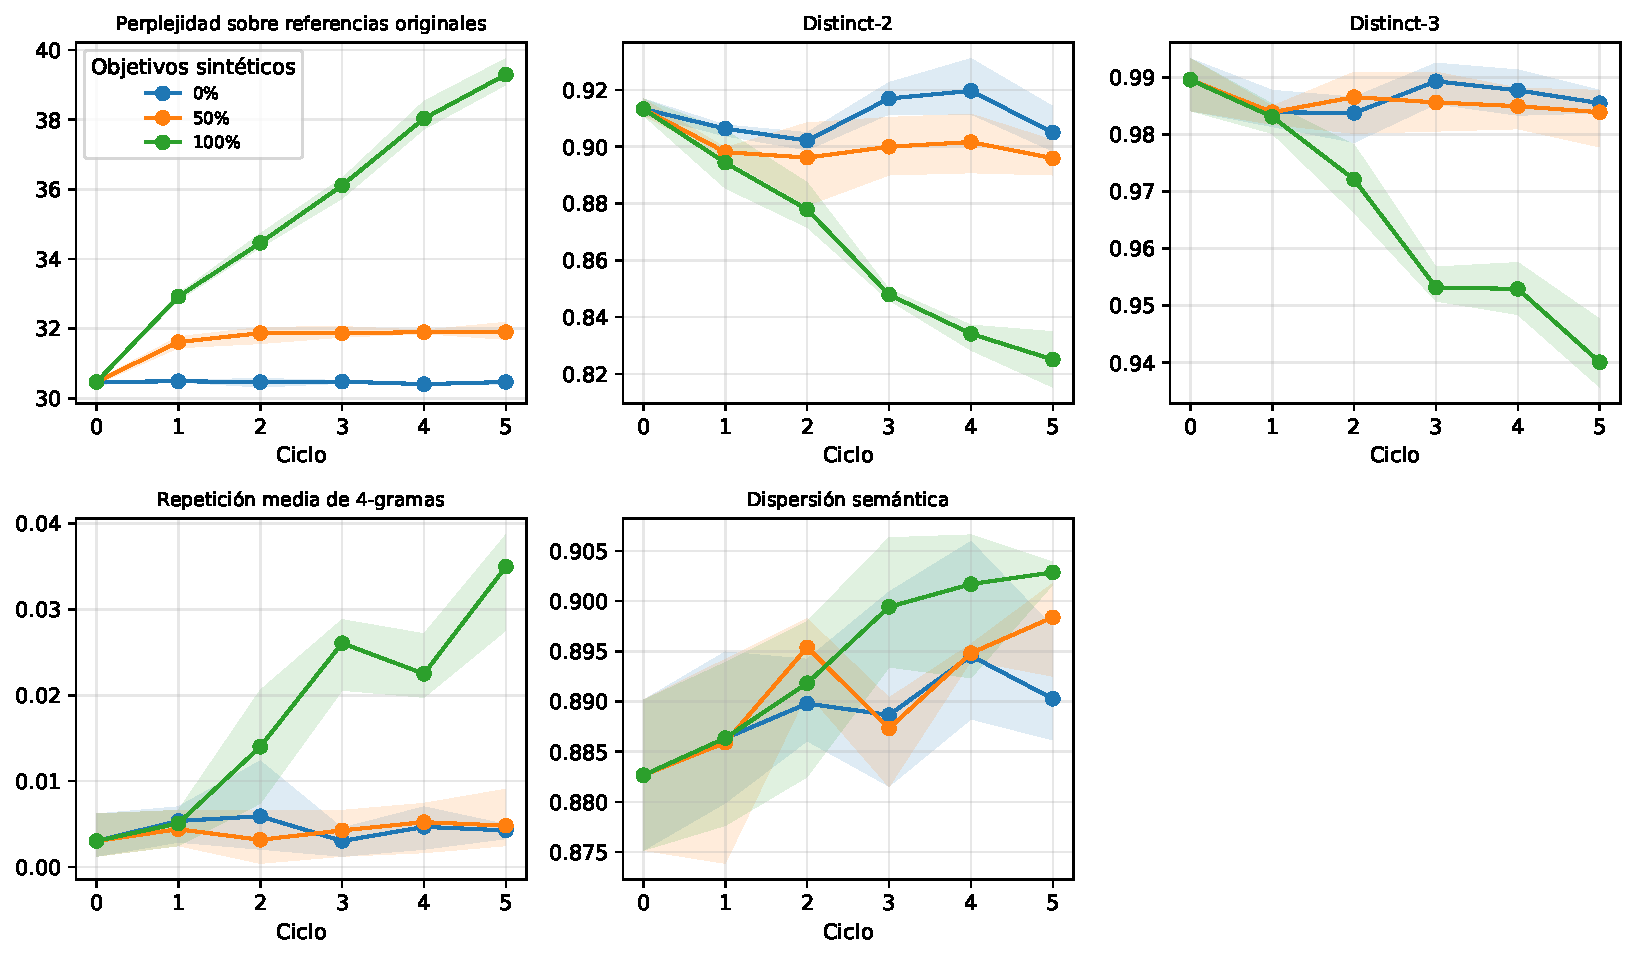
\includegraphics[width=\textwidth]{resultados_generados/figura_trayectorias.pdf}
\caption{Trayectorias por ciclo y proporción sintética: media (línea) y rango
de las tres cadenas (área sombreada). La perplejidad usa los 128 contextos
de prueba; las demás métricas corresponden al análisis complementario
\textit{post hoc} con 90 contextos comunes y \(W=30\) palabras.}
\label{fig:trayectorias}
\end{figure}

Con \(\alpha=1\), en cambio, la diversidad léxica disminuyó a partir del
segundo ciclo. Distinct-2 pasó de 0.913 en \(M_0\) a 0.825 en el ciclo 5,
una reducción cercana al 10\,\%, y Distinct-3 pasó de 0.990 a 0.940. La
repetición media de 4-gramas aumentó de 0.003 a 0.035. Aunque su valor
absoluto sigue siendo bajo para fragmentos de 30 palabras, es alrededor de
ocho veces mayor que el del control en el mismo ciclo. Las tres cadenas
coincidieron en la dirección de estos cambios.

% Generado por Experimentos/generar_resultados_latex.py desde complementario.
% No editar a mano: volver a ejecutar el script.

\begin{table}[ht]
\centering
\footnotesize
\resizebox{\textwidth}{!}{%
\begin{tabular}{l c c c c}
\hline
Métrica & $\alpha$ & $\Delta$ frente a $M_0$ & $\Delta$ frente al control & Cadenas con $\Delta>0$ \\
\hline
Perplejidad & 50\,\% & $+1.44$ [$+1.21$; $+1.67$] & $+1.43$ [$+1.18$; $+1.70$] & 3/3 \\
Perplejidad & 100\,\% & $+8.83$ [$+8.52$; $+9.36$] & $+8.83$ [$+8.50$; $+9.35$] & 3/3 \\
\hline
Distinct-2 & 50\,\% & $-0.0174$ [$-0.0268$; $-0.0088$] & $-0.0091$ [$-0.0241$; $+0.0038$] & 1/3 \\
Distinct-2 & 100\,\% & $-0.0883$ [$-0.0958$; $-0.0770$] & $-0.0799$ [$-0.0893$; $-0.0674$] & 0/3 \\
\hline
Distinct-3 & 50\,\% & $-0.0057$ [$-0.0155$; $+0.0036$] & $-0.0016$ [$-0.0099$; $+0.0028$] & 2/3 \\
Distinct-3 & 100\,\% & $-0.0495$ [$-0.0563$; $-0.0365$] & $-0.0454$ [$-0.0508$; $-0.0373$] & 0/3 \\
\hline
Repetición de 4-gramas & 50\,\% & $+0.0018$ [$-0.0037$; $+0.0074$] & $+0.0005$ [$-0.0025$; $+0.0045$] & 1/3 \\
Repetición de 4-gramas & 100\,\% & $+0.0320$ [$+0.0214$; $+0.0374$] & $+0.0307$ [$+0.0226$; $+0.0354$] & 3/3 \\
\hline
Dispersión semántica & 50\,\% & $+0.0157$ [$+0.0024$; $+0.0257$] & $+0.0081$ [$+0.0035$; $+0.0145$] & 3/3 \\
Dispersión semántica & 100\,\% & $+0.0202$ [$+0.0137$; $+0.0279$] & $+0.0126$ [$+0.0056$; $+0.0177$] & 3/3 \\
\hline
\end{tabular}}
\caption{Diferencias descriptivas en el ciclo 5: media y rango de las tres cadenas. $\Delta$ frente a $M_0$ compara con el punto inicial de la misma repetición; $\Delta$ frente al control compara con la condición $\alpha=0$ del mismo ciclo y repetición. No se calculan pruebas de significación. Salvo la perplejidad, calculada con los 128 contextos de prueba, las métricas corresponden al análisis complementario \textit{post hoc} con los 90 contextos en los que todas las etapas alcanzan $W=30$ palabras.}
\label{tab:contrastes_ciclo5}
\end{table}


Con \(\alpha=0.5\) los cambios fueron pequeños y poco consistentes.
Distinct-2 se mantuvo ligeramente por debajo del control, entre 0.896 y
0.902, pero en el ciclo 5 la diferencia frente al control fue
\(-0.009\), con un rango que incluye valores positivos. Distinct-3 y la
repetición de 4-gramas no se distinguieron del control.

\subsection{Dispersión semántica}

La dispersión semántica no disminuyó en ninguna condición. Las medias
aumentaron ligeramente en las tres proporciones: de 0.883 en \(M_0\) a
0.890 con \(\alpha=0\), 0.898 con \(\alpha=0.5\) y 0.903 con \(\alpha=1\)
en el ciclo 5. La diferencia frente al control con \(\alpha=1\) fue
positiva en las tres cadenas, de \(+0.013\) en promedio. Su magnitud es
pequeña y los rangos se traslapan en varios ciclos, por lo que no se
interpreta como un cambio robusto.

\subsection{Interacción entre proporción sintética y generaciones}

El efecto del número de ciclos dependió de la proporción sintética. Con
\(\alpha=0\) las trayectorias fueron prácticamente planas. Con
\(\alpha=0.5\) casi todo el cambio en perplejidad ocurrió en el primer
ciclo y después se mantuvo estable, de modo que añadir generaciones no
aumentó el efecto. Con \(\alpha=1\), en cambio, la perplejidad creció en
promedio unas 1.8 unidades por ciclo y la diversidad léxica y la
repetición empezaron a separarse del control a partir del segundo ciclo.
Esta dependencia se describe a partir de las trayectorias; con tres
repeticiones no se estimó un término de interacción formal.

\subsection{Variabilidad entre repeticiones}

Las tres cadenas de cada condición mostraron trayectorias muy parecidas.
En el ciclo 5, el rango de la perplejidad fue de 0.10 con \(\alpha=0\),
0.49 con \(\alpha=0.5\) y 0.75 con \(\alpha=1\), muy inferior a las
diferencias entre condiciones. En las métricas léxicas la variación entre
cadenas fue mayor en proporción: el rango de Distinct-2 fue de 0.016 con
\(\alpha=0\), 0.012 con \(\alpha=0.5\) y 0.020 con \(\alpha=1\). Esta
variabilidad es del mismo orden que la diferencia entre \(\alpha=0.5\) y
el control, lo que explica que esa comparación no sea concluyente, pero es
claramente menor que la diferencia observada con \(\alpha=1\).

\subsection{Ejemplos de continuaciones}

Los ejemplos siguientes provienen de la primera repetición y comparan, para
un mismo contexto de prueba, la generación inicial con la generación del
ciclo 5 bajo \(\alpha=1\). Se reproducen fragmentos iniciales sin
corrección; las barras indican saltos de línea.

\begin{quote}\small
\textit{\(M_0\):} «las hayas, tienden a caer en dos, que eran los procesos
de formación de las flores. En el lado basal pueden haber algo de roseta
media luna [\ldots]»\\[0.3em]
\textit{\(\alpha=1\), ciclo 5:} «las estípulas, usan frutos, tallos y hojas
en forma de flor (la inflorescencia es una flor de 16-30 cm de largo,
ovoide, 21-25 cm de largo, 3.5 cm de ancho, 5 cm de largo, 2 cm de ancho,
y 1.6 cm de largo, 1 cm de largo, 4 cm de largo, 6 cm de largo [\ldots]»
\end{quote}

\begin{quote}\small
\textit{\(M_0\):} «La geología de la República de India es considerada el
área más grande del mundo [\ldots]»\\[0.3em]
\textit{\(\alpha=1\), ciclo 5:} «La espeleología incluye dos grandes áreas
de estudio: / / / / Los países que tienen más aumento de población del mundo
[\ldots] son: / / / / En los países con más aumento de población del mundo
[\ldots] son: / / / / / / [\ldots]»
\end{quote}

Ambos textos de \(M_0\) contienen errores de contenido, lo que es esperable
en un modelo pequeño. Sin embargo, las continuaciones del ciclo 5 con
\(\alpha=1\) muestran además bucles de una misma estructura, frases
reiteradas y secuencias de saltos de línea. Estos patrones coinciden con
el aumento de la repetición de 4-gramas y de las continuaciones cortas.
Los ejemplos ilustran las mediciones y no sustituyen el análisis
cuantitativo.

\subsection{Aspectos previstos que no se evaluaron}

Dos aspectos contemplados en la planeación no se midieron en esta
ejecución. La representación de patrones poco frecuentes requería un
procedimiento específico que no se implementó, y la repetición entre
textos se aproximó únicamente mediante la dispersión semántica, sin una
medida léxica de similitud entre continuaciones. Tampoco se aplicaron
pruebas de significación; los contrastes se informan como diferencias
descriptivas entre cadenas, de acuerdo con el análisis previsto.

\section{Discusión}

\subsection{Lectura de los resultados frente a la hipótesis}

La hipótesis planteaba que el entrenamiento recurrente con contenido
sintético reduciría progresivamente la diversidad y aumentaría la
repetición, con efectos más pronunciados al aumentar la proporción
sintética y el número de generaciones. Los resultados la apoyan de forma
parcial. Bajo reemplazo total de los objetivos (\(\alpha=1\)) se observó el
patrón esperado: menor diversidad léxica, mayor repetición y una
perplejidad creciente sobre texto humano, acumulándose en cada ciclo.
El orden entre condiciones también coincidió con lo esperado: el control
se mantuvo estable, la mezcla intermedia mostró cambios moderados y el
reemplazo total, los mayores.

La hipótesis no se cumplió en dos aspectos. Con \(\alpha=0.5\) el cambio no
fue progresivo: la perplejidad aumentó en el primer ciclo y después se
estabilizó, mientras que la diversidad léxica y la repetición apenas se
separaron del control. Además, la dispersión semántica no disminuyó en
ninguna condición. Por tanto, dentro de este diseño, el deterioro observado
depende más del reemplazo completo de los datos originales que de la mera
presencia de contenido sintético, y se manifiesta en la dimensión léxica
y en la perplejidad antes que en la semántica medida.

\subsection{Relación con la literatura}

El comportamiento con \(\alpha=1\) es compatible con el deterioro descrito
por Shumailov et al.\ \cite{shumailov2024}: cada generación aprende de una
muestra del modelo anterior y asigna menor probabilidad al texto original.
El aumento sostenido de la perplejidad sobre referencias humanas es la
señal más directa de ese alejamiento. No obstante, el estudio no midió la
pérdida de eventos poco frecuentes de forma específica y abarca solo cinco
ciclos; por ello, los resultados se interpretan como una etapa temprana
compatible con el fenómeno, no como un colapso avanzado.

La estabilización con \(\alpha=0.5\) coincide con los antecedentes que
distinguen entre reemplazar los datos y conservar una parte de los
originales \cite{gerstgrasser2024,kazdan2025}. En este diseño la mitad de
los objetivos humanos permanece fija en cada ciclo, lo que parece acotar
el alejamiento respecto de la distribución original. Esta comparación es
solo cualitativa: el experimento no evaluó la acumulación de generaciones
ni corpus de tamaño creciente, que son las condiciones estudiadas en esos
trabajos.

La diferencia entre dimensiones también es coherente con Guo et al.\
\cite{guo2024}, quienes reportan reducciones más claras en la diversidad
léxica y sintáctica que en la semántica. En este estudio, la dispersión
semántica incluso aumentó ligeramente. Una explicación posible es que la
métrica compara continuaciones de 90 contextos con temas distintos, por lo
que refleja sobre todo la variedad entre temas y no la concentración dentro
de cada uno. Además, un texto que pierde coherencia con su contexto puede
parecer más disperso para el codificador sin ser más variado. Ambas
explicaciones son hipótesis y no se comprobaron en este trabajo.

Por último, la generación con \textit{top-p} de 0.95 descarta en cada ciclo
la parte menos probable de la distribución \cite{holtzman2020}. Como la
configuración de muestreo fue constante, las diferencias entre condiciones
no se deben a cambios en la decodificación. Sin embargo, este recorte
podría contribuir a que los datos sintéticos pierdan variedad de una
generación a otra, en línea con la influencia de la estrategia de
generación señalada por Drayson et al.\ \cite{drayson2025}. Comprobarlo
requeriría comparar estrategias de muestreo.

\subsection{Limitaciones}

Los resultados se limitan a un GPT-2 pequeño en español, 512 ejemplos de
Wikipedia, cinco ciclos y tres repeticiones. Con tres cadenas por condición
el análisis es descriptivo: las diferencias se informan mediante medias y
rangos, sin pruebas de significación. Que las tres cadenas coincidan en
dirección y que los rangos no se traslapen respalda la consistencia de los
cambios con \(\alpha=1\), pero no permite generalizar a otros modelos,
tamaños o dominios.

La principal limitación metodológica es la pérdida de métricas léxicas y
semánticas en 39 etapas por la regla de textos cortos. El análisis
complementario permite describir esas dimensiones, pero se definió después
de observar los datos y excluye 38 de los 128 contextos de prueba,
probablemente los más afectados. Además, \(W=30\) palabras es una ventana
breve; la dispersión semántica depende del codificador elegido; el modelo
ya había sido adaptado a Wikipedia, por lo que no puede descartarse
solapamiento con sus datos previos; y los contextos humanos se mantuvieron
incluso con \(\alpha=1\). Cada ajuste partió del mismo modelo base, de modo
que la transmisión entre generaciones ocurrió únicamente a través de los
datos. Por último, no se evaluaron la diversidad sintáctica ni la pérdida
de patrones raros con un procedimiento específico.

\section{Conclusiones}

\subsection{Respuesta a la pregunta principal}

Con un GPT-2 pequeño en español, la diversidad del contenido generado
cambió de forma distinta según la proporción de datos sintéticos. Cuando
las continuaciones originales se reemplazaron por completo, la diversidad
léxica disminuyó de manera progresiva a lo largo de los cinco ciclos
(Distinct-2 bajó cerca de un 10\,\% y Distinct-3 un 5\,\%). Al conservar
la mitad de los datos originales, los cambios fueron pequeños e
inconsistentes, y con datos originales no se observaron cambios. La
dispersión semántica, en cambio, no disminuyó en ninguna condición.

\subsection{Respuestas a las preguntas secundarias}

\begin{enumerate}
    \item \textit{Generaciones.} Con reemplazo total, la diversidad léxica
    disminuyó a partir del segundo ciclo y siguió bajando hasta el quinto.
    La dispersión semántica no se redujo; aumentó ligeramente en todas las
    condiciones.
    \item \textit{Proporción.} El efecto aumentó con la proporción
    sintética: nulo con \(\alpha=0\), moderado y estable con
    \(\alpha=0.5\) y el mayor con \(\alpha=1\). Conservar la mitad de los
    datos originales redujo considerablemente el deterioro.
    \item \textit{Repetición.} Con \(\alpha=1\) la repetición media de
    4-gramas pasó de 0.003 a 0.035 y aparecieron bucles de una misma
    estructura, frases reiteradas y saltos de línea repetidos. Con
    \(\alpha\le0.5\) la repetición no se distinguió del control.
    \item \textit{Relación entre ambos factores.} El número de
    generaciones amplificó el efecto solo bajo reemplazo total. Con la
    mezcla intermedia el cambio se concentró en el primer ciclo y después
    se estabilizó.
    \item \textit{Indicadores de model collapse.} Los rasgos que
    acompañaron el deterioro fueron el aumento sostenido de la perplejidad
    sobre texto humano, la caída de Distinct-\(n\), el aumento de la
    repetición y la aparición de continuaciones degeneradas o muy cortas.
    La dispersión semántica no resultó un indicador útil en este diseño.
\end{enumerate}

\subsection{Cumplimiento de los objetivos}

Se cumplieron los objetivos planteados dentro del alcance del
experimento. Se compararon la diversidad léxica y semántica a través de
cinco ciclos y tres proporciones, se evaluó la repetición dentro de los
textos y se describió el efecto conjunto de ambos factores. La
compatibilidad con el \textit{model collapse} se examinó considerando sus
limitaciones. El cumplimiento es descriptivo: las métricas léxicas y
semánticas proceden de un análisis complementario y la repetición entre
textos solo se aproximó mediante la dispersión semántica.

\subsection{Conclusión sobre la hipótesis}

La hipótesis se apoya parcialmente. Bajo reemplazo total de los datos
originales se observaron la disminución progresiva de la diversidad
léxica y el aumento de la repetición que se esperaban, con efectos
crecientes con las generaciones. No se apoya en la dimensión semántica
medida ni en la mezcla intermedia, donde el efecto no fue progresivo.
En conjunto, los resultados son compatibles con una etapa temprana de
\textit{model collapse} bajo reemplazo total, dentro de las condiciones
evaluadas.

\subsection{Aportaciones del estudio}

El estudio aporta una comparación controlada en español de tres
proporciones sintéticas y cinco generaciones, con tres repeticiones
independientes, ejecutada en Google Colab con una GPU T4 y documentada
con detalle suficiente para repetirla. Los resultados muestran
también que conservar una fracción fija de datos originales limita el
deterioro y que una regla de evaluación demasiado estricta puede dejar
sin medición a la mayoría de las etapas, algo que conviene prever en
estudios similares.

\subsection{Limitaciones y trabajo futuro}

Las conclusiones se limitan a un modelo pequeño, un corpus enciclopédico,
cinco ciclos y tres repeticiones, y al análisis descriptivo. Como trabajo
futuro se propone ampliar el número de ciclos y repeticiones, evaluar
otros modelos, tareas e idiomas, comparar estrategias de muestreo y
políticas de acumulación, incorporar medidas de diversidad sintáctica y
de pérdida de patrones raros, y definir desde el inicio un tratamiento de
las salidas cortas que no invalide etapas completas.


\clearpage
\phantomsection
\addcontentsline{toc}{section}{Referencias}
\begin{thebibliography}{99}

\bibitem{shumailov2024}
Shumailov, I., Shumaylov, Z., Zhao, Y., et al.
\textit{AI models collapse when trained on recursively generated data}.
Nature, 631, 755--759, 2024.
\url{https://doi.org/10.1038/s41586-024-07566-y}

\bibitem{kazdan2025}
Kazdan, J., Schaeffer, R., Dey, A., Gerstgrasser, M., Rafailov, R.,
Donoho, D. L., y Koyejo, S.
\textit{Collapse or Thrive: Perils and Promises of Synthetic Data in a
Self-Generating World}.
Proceedings of the 42nd International Conference on Machine Learning,
PMLR, 267, 29469--29494, 2025.
\url{https://proceedings.mlr.press/v267/kazdan25a.html}

\bibitem{bengio2003}
Bengio, Y., Ducharme, R., Vincent, P., y Jauvin, C.
\textit{A Neural Probabilistic Language Model}.
Journal of Machine Learning Research, 3, 1137--1155, 2003.
\url{https://jmlr.org/papers/v3/bengio03a.html}

\bibitem{vaswani2017}
Vaswani, A., Shazeer, N., Parmar, N., et al.
\textit{Attention Is All You Need}.
Advances in Neural Information Processing Systems, 30, 2017.
\url{https://papers.nips.cc/paper_files/paper/2017/hash/3f5ee243547dee91fbd053c1c4a845aa-Abstract.html}

\bibitem{holtzman2020}
Holtzman, A., Buys, J., Du, L., Forbes, M., y Choi, Y.
\textit{The Curious Case of Neural Text Degeneration}.
International Conference on Learning Representations, 2020.
Preprint inicial: arXiv:1904.09751, 2019.
\url{https://arxiv.org/abs/1904.09751}

\bibitem{wang2023selfinstruct}
Wang, Y., Kordi, Y., Mishra, S., Liu, A., Smith, N. A.,
Khashabi, D., y Hajishirzi, H.
\textit{Self-Instruct: Aligning Language Models with Self-Generated Instructions}.
Proceedings of ACL, 13484--13508, 2023.
\url{https://aclanthology.org/2023.acl-long.754/}

\bibitem{zhu2025}
Zhu, X., Cheng, D., Li, H., et al.
\textit{How to Synthesize Text Data without Model Collapse?}.
Proceedings of ICML, PMLR, 267, 79746--79771, 2025.
\url{https://proceedings.mlr.press/v267/zhu25d.html}

\bibitem{drayson2025}
Drayson, G., Yilmaz, E., y Lampos, V.
\textit{Machine-generated text detection prevents language model collapse}.
Proceedings of EMNLP, 29657--29673, 2025.
\url{https://aclanthology.org/2025.emnlp-main.1506/}

\bibitem{guo2024}
Guo, Y., Shang, G., Vazirgiannis, M., y Clavel, C.
\textit{The Curious Decline of Linguistic Diversity:
Training Language Models on Synthetic Text}.
Findings of NAACL, 3589--3604, 2024.
\url{https://aclanthology.org/2024.findings-naacl.228/}

\bibitem{reimers2019}
Reimers, N., y Gurevych, I.
\textit{Sentence-BERT: Sentence Embeddings using Siamese BERT-Networks}.
Proceedings of EMNLP-IJCNLP, 3982--3992, 2019.
\url{https://aclanthology.org/D19-1410/}

\bibitem{li2016}
Li, J., Galley, M., Brockett, C., Gao, J., y Dolan, B.
\textit{A Diversity-Promoting Objective Function for Neural Conversation Models}.
Proceedings of NAACL-HLT, 110--119, 2016.
\url{https://aclanthology.org/N16-1014/}

\bibitem{zhu2018texygen}
Zhu, Y., Lu, S., Zheng, L., Guo, J., Zhang, W., Wang, J., y Yu, Y.
\textit{Texygen: A Benchmarking Platform for Text Generation Models}.
Proceedings of SIGIR, 1097--1100, 2018.
\url{https://doi.org/10.1145/3209978.3210080}

\bibitem{pillutla2021}
Pillutla, K., Swayamdipta, S., Zellers, R., Thickstun, J.,
Welleck, S., Choi, Y., y Harchaoui, Z.
\textit{MAUVE: Measuring the Gap Between Neural Text and Human Text
using Divergence Frontiers}.
Advances in Neural Information Processing Systems, 34, 2021.
\url{https://papers.nips.cc/paper_files/paper/2021/hash/260c2432a0eecc28ce03c10dadc078a4-Abstract.html}

\bibitem{suresh2025}
Suresh, A. T., Thangaraj, A., y Khandavally, A. N. K.
\textit{Rate of Model Collapse in Recursive Training}.
Proceedings of the 28th International Conference on Artificial Intelligence
and Statistics, PMLR, 258, 1396--1404, 2025.
\url{https://proceedings.mlr.press/v258/suresh25a.html}

\bibitem{gerstgrasser2024}
Gerstgrasser, M., Schaeffer, R., Dey, A., et al.
\textit{Is Model Collapse Inevitable? Breaking the Curse of Recursion
by Accumulating Real and Synthetic Data}.
Preprint arXiv:2404.01413v2, 2024.
\url{https://doi.org/10.48550/arXiv.2404.01413}

\bibitem{spanishmodelcard}
Datificate. \textit{Model card: gpt2-small-spanish}.
Ficha del modelo consultada el 9 de noviembre de 2026.
\url{https://huggingface.co/datificate/gpt2-small-spanish}

\bibitem{wikipediacard}
Wikimedia. \textit{Dataset card: Wikipedia}, configuración 20231101.es.
Ficha del conjunto consultada el 9 de noviembre de 2026.
\url{https://huggingface.co/datasets/wikimedia/wikipedia}

\bibitem{multilingualcard}
Sentence Transformers. \textit{Model card: paraphrase-multilingual-MiniLM-L12-v2}.
Ficha del codificador consultada el 9 de noviembre de 2026.
\url{https://huggingface.co/sentence-transformers/paraphrase-multilingual-MiniLM-L12-v2}

\end{thebibliography}

\clearpage
\appendix
\renewcommand{\thesection}{\Alph{section}}

\section{Configuración completa del experimento}

\begin{table}[ht]
\centering
\footnotesize
\resizebox{\textwidth}{!}{%
\begin{tabular}{l l}
\hline
Parámetro & Valor \\
\hline
Modelo base & \texttt{datificate/gpt2-small-spanish} (rev.\ \texttt{02e30923}) \\
Corpus & \texttt{wikimedia/wikipedia}, \texttt{20231101.es} (rev.\ \texttt{b04c8d1c}) \\
Codificador semántico & \texttt{paraphrase-multilingual-MiniLM-L12-v2} (rev.\ \texttt{e8f8c211}) \\
Artículos recorridos & 2000 (prefijo en streaming) \\
Semilla de partición y del estudio & 20261109 \\
Ejemplos de entrenamiento / validación / prueba & 512 / 128 / 128 \\
Tokens de contexto / objetivo & 64 / 128 \\
Proporciones sintéticas \(\alpha\) & 0, 0.5 y 1 \\
Ciclos y repeticiones & 5 ciclos, 3 repeticiones (48 ajustes) \\
Optimizador & AdamW, \(2\times10^{-5}\), \(\beta=(0.9,\,0.999)\), \(\epsilon=10^{-8}\), decaimiento 0.01 \\
Lote & efectivo 8 (microlotes de 2), 1 época, 64 actualizaciones \\
Recorte de gradiente & norma 1.0, float32, sin \textit{scheduler} \\
Generación & temperatura 1.0, \textit{top-p} 0.95, 128 tokens sin IDs especiales \\
Longitud léxica \(W\) & máximo 32; valor fijado con validación: 30 \\
Límite del codificador & 128 \textit{wordpieces} \\
Entorno & Colab, Tesla T4, CUDA 13.0, Python 3.13.16, PyTorch 2.14.1, Transformers 5.22.2 \\
\hline
\end{tabular}}
\caption{Configuración congelada en el protocolo del estudio principal.}
\label{tab:configuracion}
\end{table}

Los contextos de entrada son los primeros 64 tokens de una ventana
seleccionada al azar, con semilla fija, en cada artículo de Wikipedia;
no se utilizaron instrucciones. Los identificadores de los artículos y las ventanas exactas se
registraron para poder reconstruir el corpus.

\section{Tablas completas de resultados}

Las tablas siguientes presentan, por ciclo y proporción, las métricas
del análisis complementario. La tabla de perplejidad se presentó en la
sección de resultados.

% Generado por Experimentos/generar_resultados_latex.py desde complementario.
% No editar a mano: volver a ejecutar el script.

\begin{table}[ht]
\centering
\footnotesize
\begin{tabular}{c c c c}
\hline
Ciclo & $\alpha=0$ & $\alpha=0.5$ & $\alpha=1$ \\
\hline
0 ($M_0$) & \multicolumn{3}{c}{$0.9133$ [$0.9111$; $0.9169$]} \\
1 & $0.9064$ [$0.9038$; $0.9077$] & $0.8981$ [$0.8958$; $0.8996$] & $0.8944$ [$0.8854$; $0.9057$] \\
2 & $0.9022$ [$0.8989$; $0.9050$] & $0.8962$ [$0.8793$; $0.9084$] & $0.8779$ [$0.8716$; $0.8874$] \\
3 & $0.9170$ [$0.9115$; $0.9226$] & $0.9000$ [$0.8900$; $0.9103$] & $0.8479$ [$0.8460$; $0.8498$] \\
4 & $0.9197$ [$0.9115$; $0.9310$] & $0.9017$ [$0.8908$; $0.9115$] & $0.8341$ [$0.8284$; $0.8372$] \\
5 & $0.9050$ [$0.8985$; $0.9142$] & $0.8959$ [$0.8900$; $0.9023$] & $0.8250$ [$0.8153$; $0.8349$] \\
\hline
\end{tabular}
\caption{Distinct-2: media y rango [mínimo; máximo] de las tres cadenas por ciclo y proporción sintética $\alpha$. $M_0$ es compartido por las tres proporciones dentro de cada repetición. Salvo la perplejidad, calculada con los 128 contextos de prueba, las métricas corresponden al análisis complementario \textit{post hoc} con los 90 contextos en los que todas las etapas alcanzan $W=30$ palabras.}
\label{tab:medias_distinct_2}
\end{table}

% Generado por Experimentos/generar_resultados_latex.py desde complementario.
% No editar a mano: volver a ejecutar el script.

\begin{table}[ht]
\centering
\footnotesize
\begin{tabular}{c c c c}
\hline
Ciclo & $\alpha=0$ & $\alpha=0.5$ & $\alpha=1$ \\
\hline
0 ($M_0$) & \multicolumn{3}{c}{$0.9896$ [$0.9841$; $0.9933$]} \\
1 & $0.9839$ [$0.9813$; $0.9877$] & $0.9839$ [$0.9817$; $0.9849$] & $0.9831$ [$0.9802$; $0.9853$] \\
2 & $0.9837$ [$0.9786$; $0.9865$] & $0.9865$ [$0.9802$; $0.9909$] & $0.9721$ [$0.9663$; $0.9782$] \\
3 & $0.9893$ [$0.9853$; $0.9925$] & $0.9856$ [$0.9806$; $0.9909$] & $0.9532$ [$0.9508$; $0.9567$] \\
4 & $0.9877$ [$0.9833$; $0.9913$] & $0.9849$ [$0.9810$; $0.9881$] & $0.9529$ [$0.9484$; $0.9575$] \\
5 & $0.9854$ [$0.9837$; $0.9877$] & $0.9839$ [$0.9778$; $0.9877$] & $0.9401$ [$0.9357$; $0.9476$] \\
\hline
\end{tabular}
\caption{Distinct-3: media y rango [mínimo; máximo] de las tres cadenas por ciclo y proporción sintética $\alpha$. $M_0$ es compartido por las tres proporciones dentro de cada repetición. Salvo la perplejidad, calculada con los 128 contextos de prueba, las métricas corresponden al análisis complementario \textit{post hoc} con los 90 contextos en los que todas las etapas alcanzan $W=30$ palabras.}
\label{tab:medias_distinct_3}
\end{table}

% Generado por Experimentos/generar_resultados_latex.py desde complementario.
% No editar a mano: volver a ejecutar el script.

\begin{table}[ht]
\centering
\footnotesize
\begin{tabular}{c c c c}
\hline
Ciclo & $\alpha=0$ & $\alpha=0.5$ & $\alpha=1$ \\
\hline
0 ($M_0$) & \multicolumn{3}{c}{$0.0030$ [$0.0012$; $0.0062$]} \\
1 & $0.0053$ [$0.0029$; $0.0070$] & $0.0044$ [$0.0025$; $0.0066$] & $0.0051$ [$0.0025$; $0.0066$] \\
2 & $0.0059$ [$0.0021$; $0.0123$] & $0.0032$ [$0.0004$; $0.0066$] & $0.0140$ [$0.0074$; $0.0206$] \\
3 & $0.0030$ [$0.0012$; $0.0045$] & $0.0043$ [$0.0012$; $0.0066$] & $0.0261$ [$0.0206$; $0.0288$] \\
4 & $0.0047$ [$0.0021$; $0.0070$] & $0.0052$ [$0.0016$; $0.0074$] & $0.0225$ [$0.0198$; $0.0272$] \\
5 & $0.0043$ [$0.0033$; $0.0049$] & $0.0048$ [$0.0025$; $0.0091$] & $0.0350$ [$0.0276$; $0.0387$] \\
\hline
\end{tabular}
\caption{Repetición media de 4-gramas: media y rango [mínimo; máximo] de las tres cadenas por ciclo y proporción sintética $\alpha$. $M_0$ es compartido por las tres proporciones dentro de cada repetición. Salvo la perplejidad, calculada con los 128 contextos de prueba, las métricas corresponden al análisis complementario \textit{post hoc} con los 90 contextos en los que todas las etapas alcanzan $W=30$ palabras.}
\label{tab:medias_repeat_4_mean}
\end{table}

% Generado por Experimentos/generar_resultados_latex.py desde complementario.
% No editar a mano: volver a ejecutar el script.

\begin{table}[ht]
\centering
\footnotesize
\begin{tabular}{c c c c}
\hline
Ciclo & $\alpha=0$ & $\alpha=0.5$ & $\alpha=1$ \\
\hline
0 ($M_0$) & \multicolumn{3}{c}{$0.8827$ [$0.8752$; $0.8901$]} \\
1 & $0.8863$ [$0.8799$; $0.8949$] & $0.8859$ [$0.8739$; $0.8942$] & $0.8864$ [$0.8777$; $0.8939$] \\
2 & $0.8898$ [$0.8861$; $0.8942$] & $0.8954$ [$0.8909$; $0.8982$] & $0.8918$ [$0.8825$; $0.8980$] \\
3 & $0.8886$ [$0.8816$; $0.9009$] & $0.8873$ [$0.8815$; $0.8904$] & $0.8994$ [$0.8934$; $0.9063$] \\
4 & $0.8945$ [$0.8883$; $0.9059$] & $0.8948$ [$0.8941$; $0.8957$] & $0.9017$ [$0.8923$; $0.9066$] \\
5 & $0.8903$ [$0.8862$; $0.8974$] & $0.8984$ [$0.8925$; $0.9018$] & $0.9029$ [$0.9017$; $0.9039$] \\
\hline
\end{tabular}
\caption{Dispersión semántica: media y rango [mínimo; máximo] de las tres cadenas por ciclo y proporción sintética $\alpha$. $M_0$ es compartido por las tres proporciones dentro de cada repetición. Salvo la perplejidad, calculada con los 128 contextos de prueba, las métricas corresponden al análisis complementario \textit{post hoc} con los 90 contextos en los que todas las etapas alcanzan $W=30$ palabras.}
\label{tab:medias_semantic_dispersion}
\end{table}



\end{document}
